\section{Resultater}
I dette afsnit samles der op på resultaterne gruppen har opnået gennem projektforløbet. Her vil der blive beskrevet resultater for de enkelte moduler gruppen har implementeret. Til sidst bliver der knyttet en kommentar til det samlerede resultat. Der vil i afsnittet blive henvist til testresultater dokumenteret i hhv. "Enhedstest", "Integrationstest" og "Accepttest".

\subsection{KI}
Kontrolinterfacet er fuldt implementeret og har opfyldt alle enhedstests for modulet. TCP- og UART-kommunikationen er udviklet i Qt med API'er specifikke for Qt. På trods af at der er flere steder hvor der godt kunne ske forbedringer (se afsnit \fxnote{indsæt reference til forbedringer}, så er slutresultatet, med tanke på arbejdsbyrden set i forhold til at opgaven har været en enkeltmandsopgave, et tilfredsstillende resultat.\\

\subsection{Database og webinterface}
Database og Webinterfacet er fuldt implementeret. I database modulet er serveren fuldt kørende og har en stabil forbindelse med KI via TCP. Serveren er i stand til at motage data fra KI. Benytte en dekryptering til at omsætte hældningen fra SM til grader og gemme denne som en tekstfil. Lagring direkte til MySQL blev aldrig implementeret grundet broplemer med MySQL driver. Selve MySQL databasen er fuldt kørende og fungere fejlfrit. \\
Webinterfacet er fuldt implementeret og ved opstart af webinterfacet fungere bruger adgangskoden næsten korrekt. Der opstår et problem ved fejl password hvor brugeren får en hvid side i stedet for igen at blive bedt om nyt password men får dog ikke adgang til data. Ved korrekt adgangskode får brugeren mulighed for at vælge skib og få dennes data frem. Ved inndlæsning af data siden bliver tekstfilen som serveren genereret hentet. Data bliver taget ud fra den og gemt i MySQL databsen og filen slettet. Alle data bliver hentet fra MySQL databasen med de nyeste øverst. Siden checker hvert 5 sekund om der er ny data. Hvis der ikke er ny data foretages der intet.

\subsection{SM}
SM modulet er fuldt implementeret, men ikke finjusteret. Forbindelsen til KI er fuldt funktionel. Forbindelsen til VBTE virker 95\% af tiden. Automatisk hældningsregulering er implementeret, men da niveaumålinger ikke modtages fra VBTE modulet er det ikke muligt at tømme tankene inden vi fylder i den anden tank. Prototypen er modulet er monteret med 7 LED's der bruges til fejlfinding. Prototypen er også lagt ud på print med indeholdende levelkonvertering og I2C pull-up modstande.

\subsection{VBTE}
VBTE modulet nåede aldrig at komme til at fungere optimalt. Efter at have implementeret ultralydsafstandsensoren fandt jeg ud af at det ikke fungerede ret godt over særligt lange afstande (i hvert fald i mit design). Men under kontrolerede forhold i laboratoriet lykkedes det at få flotte detektioner på ultralydsafstandssensoren som kan ses på \textit{figur \ref{res:ultraresultater}}.
\begin{figure}[H]
\centering
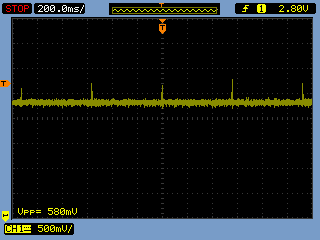
\includegraphics[width = .5\textwidth]{billeder/mixer2}
\label{res:ultraresultater}
\caption{Detektioner af ultralydsafstandssensoren med faste intervaller.}
\end{figure}
Derudover virkede I2C delen, dog med fejl på data i nogle transmissioner. Det vides ikke om det er et normalt problem ved I2C eller om det havde noget at gøre med vores system. Til sidst er der udlagt print til VBTE'en, en 2x16 LCD skærm til test samt dipswitches og knap til at skifte I2C adresse mens systemet kører. 

\subsection{Strømforsyning}
Strømforsyning er fuldt implementeret, i testen er der blevet brugt effekt modstande som load, en labitoriestrømforsyning og et voltmeter. Enhedstesten er blevet godkendt. Vitale dele på strømforsyningen bliver dog noget varme ved fuld load på udgangen, men da det med stor sandsynlighed sjælende vil ske, ses det ikke som et problem. Strømforsyningen er implementeret med SM og VBTE. Derudover er der udlagt et print med 12V og 5V forsyning.

\subsection{Samlede resultat og vurdering af resultater}
Til de samlede resultater har gruppen udarbejdet en tabel der viser hvordan test's er gået helt nede fra enhedstest til accepttest. For detaljer om de enkelte test henvises til "Enhedstest", "Integrationstest" og "Accepttest". Testresultaterne er opdelt i fire katagorier som angivet i tabellen :
\begin{table}[H]
\centering
\begin{tabular}{cccc}
\hline
Godkendt 	& Delvist godkendt 	& Ikke godkendt & Ikke testet \\
\cmidrule(r){1-1} \cmidrule(r){2-2} \cmidrule(r){3-3} \cmidrule(r){4-4}
$\surd$		& $\times$		& $\div$ & $\diamond$	\\\hline
\end{tabular}
\caption{Testgodkendelseskatagorier}
\end{table}
\begin{table}[H]
\centering
\begin{tabular}{llllllll}
\hline
\multicolumn{1}{c}{Test} & \multicolumn{7}{c}{Test case ID}\\
\cmidrule(r){1-1} \cmidrule(r){2-8} 
\textbf{Enhedstest software} & 1 & 2 & 3 & 4 & 5 & 6 & 7\\
\hline
\phantom{mm}KI  		& $\surd$ & $\surd$ & $\surd$ & $\surd$ & $\surd$ \\
\phantom{mm}Database  	& $\surd$ & $\surd$ & $\surd$ & $\surd$ & $\surd$ \\
\phantom{mm}SM			& $\surd$ & $\surd$ & $\surd$ & $\surd$ & $\surd$ &  $\surd$ & $\surd$\\
\phantom{mm}VBTE  		& $\surd$ & $\surd$ & $\surd$ & $\surd$ & $\surd$ \\ 
\textbf{Enhedstest hardware} \\
\hline
\phantom{mm}SM			& $\surd$ & $\surd$\\
\phantom{mm}VBTE  		& $\surd$ & $\surd$ & $\times$ \\ 
\phantom{mm}Strømforsyning & $\surd$ & $\surd$ & $\surd$\\
\hline
\textbf{Integrationstest} & $\surd$ & $\surd$ & $\surd$ & $\surd$ & $\surd$ & $\surd$\\
\textbf{Accepttest} & $\surd$ & $\times$ & $\times$ & $\surd$ & $\surd$ & $\surd$\\
\hline
\end{tabular}
\caption{Samlet tabel med alle resultater}
\label{table:alle test samlet}
\end{table}
Som tabellen illustrerer er der blevet implementeret en masse funktionaliteter som er blevet godkendt gennem enhedstest. Dog var der problemer med afstandsmåling på VBTE og denne testcase kunne derfor kun delvist godkendes.\\
Integration af systemets enheder er blevet godkendt.\\
Grundet problemer med afstandmåling på VBTE kan Acceptest case 2 og 3 blive mere end delvist godkendt.\\